\documentclass[11pt]{article}
\usepackage{graphicx}
\usepackage{amsmath}
\usepackage{geometry}

\geometry{margin=1in}

\title{Quantization and Sampling Noise Analysis in SAR ADCs}
\author{}
\date{}

\begin{document}

\maketitle

\section{Quantization Noise in ADCs}

\begin{figure}[htbp]
  \centering
  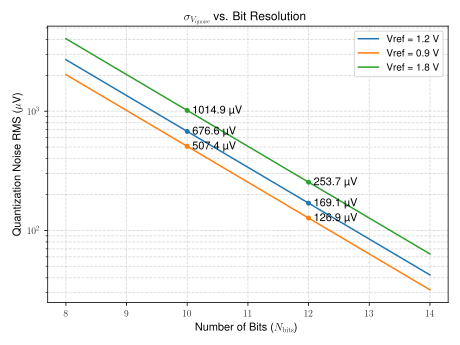
\includegraphics[width=0.8\textwidth,keepaspectratio]{../build/qnoise.pdf}
  \caption{Quantization noise characteristics in ADCs}
\end{figure}

The quantization noise standard deviation is given by:

\begin{equation}
\sigma_{V_{\mathrm{qnoise}}} = \frac{2 V_\mathrm{ref}}{2^N \sqrt{12}}
\end{equation}

\section{Sampling Noise in SAR ADCs}

\begin{figure}[htbp]
  \centering
  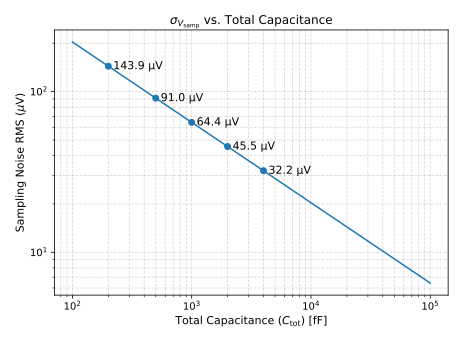
\includegraphics[width=0.8\textwidth,keepaspectratio]{../build/sampnoise.pdf}
  \caption{Sampling noise analysis in SAR ADCs}
\end{figure}

\section{ENOB vs Total Capacitance: Sampling Noise}

\begin{figure}[htbp]
  \centering
  \begin{minipage}{0.48\textwidth}
    \centering
    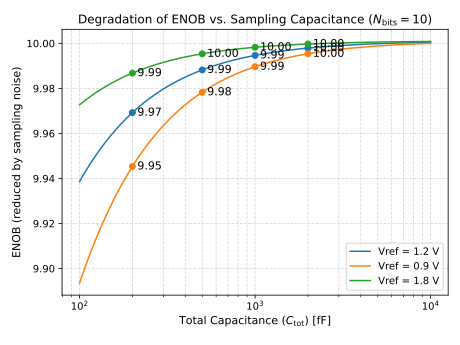
\includegraphics[width=\linewidth,keepaspectratio]{../build/enob_vs_Ctot_10bit.pdf}
    \caption{10-bit ENOB vs $C_{tot}$}
  \end{minipage}
  \hfill
  \begin{minipage}{0.48\textwidth}
    \centering
    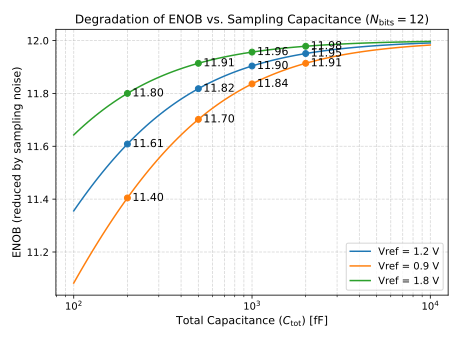
\includegraphics[width=\linewidth,keepaspectratio]{../build/enob_vs_Ctot_12bit.pdf}
    \caption{12-bit ENOB vs $C_{tot}$}
  \end{minipage}
\end{figure}

\section{Unit Fringe Capacitor}

Metal-on-metal (MOM) capacitor characteristics for 65nm CMOS process:

\begin{itemize}
  \item 1 layer: $0.31~\mathrm{fF}/\mu\mathrm{m}^2$
  \item 2 layers: $0.62~\mathrm{fF}/\mu\mathrm{m}^2$
  \item 3 layers: $0.93~\mathrm{fF}/\mu\mathrm{m}^2$
\end{itemize}

Pelgrom matching coefficient: $\sigma(\Delta C/C) = 0.85\% \times \sqrt{C~[\mathrm{fF}]}$

\begin{figure}[htbp]
  \centering
  \begin{minipage}{0.48\textwidth}
    \centering
    \includegraphics[width=\linewidth,keepaspectratio]{./images/cdac_unit_cell_3d.png}
    \caption{3D view of CDAC unit cell}
  \end{minipage}
  \hfill
  \begin{minipage}{0.48\textwidth}
    \centering
    \includegraphics[width=\linewidth,keepaspectratio]{./images/cdac_unit_cell.png}
    \caption{CDAC unit cell layout}
  \end{minipage}
\end{figure}

\section{Expected Mismatch and DNL Noise}

\begin{figure}[htbp]
  \centering
  \begin{minipage}{0.48\textwidth}
    \centering
    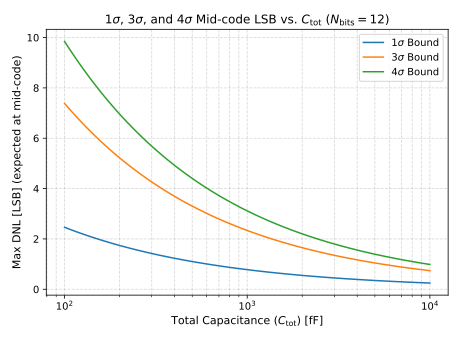
\includegraphics[width=\linewidth,keepaspectratio]{../build/expected_mismatch_12bit.pdf}
    \caption{Expected mismatch (12-bit)}
  \end{minipage}
  \hfill
  \begin{minipage}{0.48\textwidth}
    \centering
    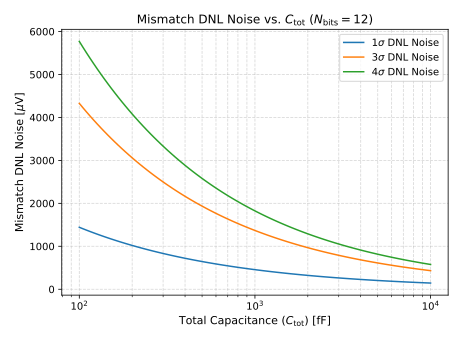
\includegraphics[width=\linewidth,keepaspectratio]{../build/mismatch_dnl_noise_12bit.pdf}
    \caption{DNL noise from mismatch (12-bit)}
  \end{minipage}
\end{figure}

\section{ENOB Comparison: Sampling Noise vs Mismatch DNL Noise}

\begin{figure}[htbp]
  \centering
  \begin{minipage}{0.48\textwidth}
    \centering
    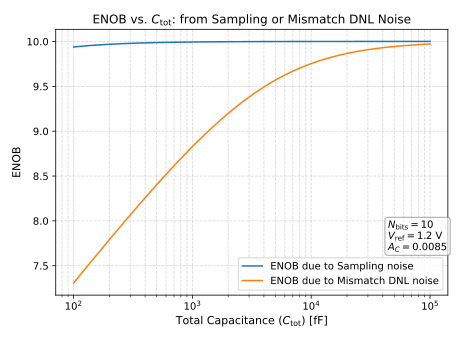
\includegraphics[width=\linewidth,keepaspectratio]{../build/enob_vs_Ctot_10bit_compare.pdf}
    \caption{10-bit comparison}
  \end{minipage}
  \hfill
  \begin{minipage}{0.48\textwidth}
    \centering
    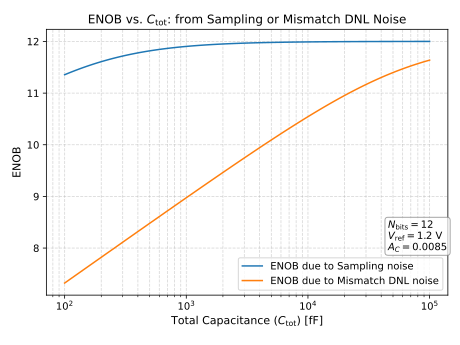
\includegraphics[width=\linewidth,keepaspectratio]{../build/enob_vs_Ctot_12bit_compare.pdf}
    \caption{12-bit comparison}
  \end{minipage}
\end{figure}

\textbf{Note:} Assuming a worst case $3\sigma$ variation, corresponding to roughly 1 in 300 ADCs.

\section{CDAC Array Overview}

The complete CDAC array specifications:

\begin{align}
\text{Total Area} &= 1940~\mu\mathrm{m}^2 \\
C_\mathrm{tot} &= 1.4~\mathrm{pF}
\end{align}

\begin{figure}[htbp]
  \centering
  \begin{minipage}{0.48\textwidth}
    \centering
    \includegraphics[width=\linewidth,keepaspectratio]{./images/cdac_array_3d.png}
    \caption{3D view of CDAC array}
  \end{minipage}
  \hfill
  \begin{minipage}{0.48\textwidth}
    \centering
    \includegraphics[width=\linewidth,keepaspectratio]{./images/cdac_array.png}
    \caption{CDAC array layout}
  \end{minipage}
\end{figure}

\end{document}